\documentclass[12pt,a4paper,oneside]{article}

\usepackage[utf8]{inputenc}
\usepackage[T1]{fontenc}
\usepackage[french]{babel}
\usepackage{amssymb}
\usepackage{amsmath}
\usepackage{graphicx}
\usepackage{float}
\usepackage{mathtools}


\author{Matteo Besançon}
\title {Préparation examens outils formels}
\date{\today}
\begin{document}
	\maketitle

\section{Formalisme RdP}
	\subsubsection*{1. Définition formelle de la structure des RdP (syntaxe)}
		\begin{description}
			\item [P] Places (Rond)
			\item [T] Transitions (Rectangle)
			\item [ ] Jeton (point noir)
		\end{description}

		Un réseau R est un quadruplet R

		$$R = (P,T, Entree, Sortie)$$

		Pour $p \in P$ et $t \in T$ si :
		\begin{itemize}
			\item $k = Entree(p,t) > 0$ $p$ est une place d'entrée de $t$ et $t$ est une place de sortie de $p$
			\item $k = Sortie(p,t) > 0$ $p$ est une place de sortie de $t$ et $t$ est une place d'entrée de $p$
		\end{itemize}

		On a les représentations matricielles suivantes :

		\begin{figure}[H]
			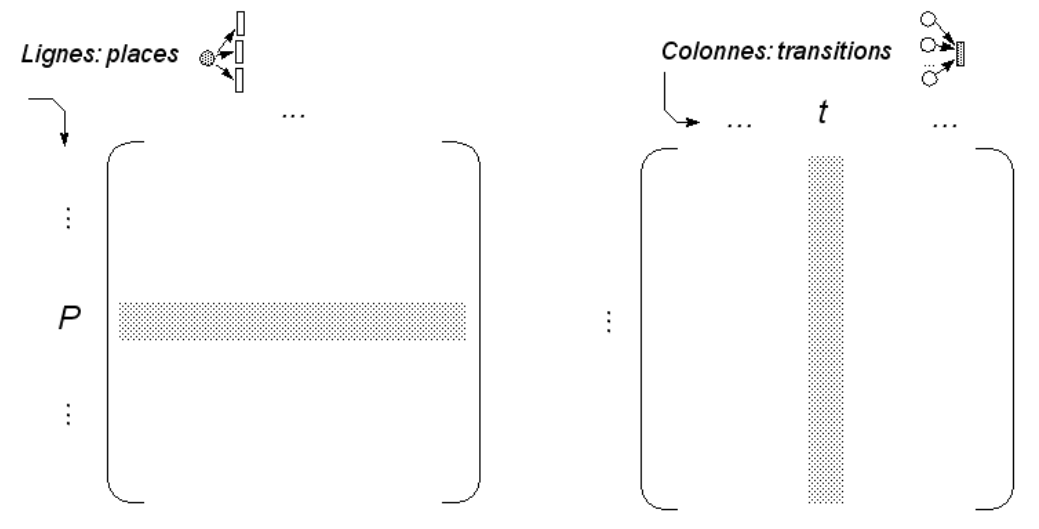
\includegraphics[scale = 0.4]{./img/entree.png}
			\centering
			\caption{Matrice d'entrée et de sortie}
			\label{entreeSortie}
		\end{figure}

		Par exemple avec le RdP suivant :

		\begin{figure}[h]
			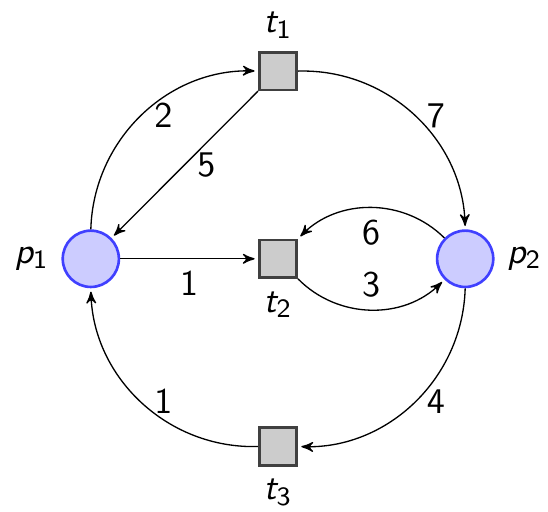
\includegraphics[scale = 0.5]{./img/exrdp.png}
			\centering
			\caption{RdP d'exemple}
			\label{exrdp}
		\end{figure}

		On a donc les matrices suivantes :
		$$Entree = \begin{bmatrix}
			2 & 1 & 0 \\
			0 & 6 & 4
		\end{bmatrix}
		Sortie = \begin{bmatrix}
			5 & 0 & 1 \\
			7 & 3 & 0
		\end{bmatrix}$$

		L'état d'un RdP est appelé un marquage $M:P\to \mathbb{N}$ souvent le marquage initial est noté $M_0$

		Pour la figure \ref{exrdp} on a la matrice de marquage:
		$$M = \begin{bmatrix}
			2\\
			3
		\end{bmatrix}$$
	\subsubsection*{2. Définition formelle des règles de franchissabilité des transitions (sémantique)}
		Y a un jeton et paf plus de jeton !!

	\subsubsection*{3. Utilisation de l’algèbre linéaire pour définir la franchissabilité des transitions}

	Une transition $t$ est franchissable (tirable) si :
	$$\forall p \in P,\ M(p) \geq Entree(p,t)$$
	par exemple pour la figure \ref{exrdp} $t_1$ est tirable et $t_3$ ne l'est pas.

	Après avoir tiré la transition $t$ on a :
	$$\forall p \in P,\ M'(p) = M(p) - Entree(p,t) + Sortie(p,t)$$

	On a la notation $M \xrightarrow[]{t} M'$

	On note $C$ la matrice d'incidence du réseau définie par
	$$\forall p \in P,\ \forall t \in t,\ C(p,t) = Sortie(p,t) - Entree(p,t)$$

	donc
	$$M' = M + C(\dots,t)$$

	Si on reprends l'expemple de la figure \ref{exrdp}
	$$C = \begin{bmatrix}
		3 & -1 & 1 \\
		7 & -3 & -4
	\end{bmatrix}$$

	Et donc si on tire $t_1$
	$$M' = M + C(\dots,t_1) =
	\begin{pmatrix}
		2\\
		3
	\end{pmatrix}
	+
	\begin{bmatrix}
		3 & -1 & 1 \\
		7 & -3 & -4
	\end{bmatrix}
	\begin{pmatrix}
		1\\
		0\\
		0
	\end{pmatrix}
	=
	\begin{pmatrix}
		5\\
		10
	\end{pmatrix}
	$$

\subsubsection*{4. Propriétés des séquences de franchissements, vecteur caractéristique et équation fondamentale}


\end{document}
